% !TeX root = ../main.tex
% Add the above to each chapter to make compiling the PDF easier in some editors.

\chapter{3D Pose Estimation}\label{chapter:3Dpose}

This chapter examines the 3D pose estimation problem. In this chapter we train three models and examine what each design choice and present the qualitative and quantitative results. All models take the x-y pixel location as input and produce 3D joint locations in the mm space. While the second and third model take the input in sequences the first model takes in frame by frame. The main problems we aim to solve in 3D pose estimation are:
\begin{itemize}
    \item Being invariant to the viewpoint of the camera
    \item Dealing with missing joints in the sequence
    \item Having a noisy 2D pose estimates as input
    \item Being invariant to changes in apparent size of the person when he or she gets close or farther away from the camera
\end{itemize}

All models are written in Tensorflow \parencite{abadi2016tensorflow} which is an efficient and popular Deep Learning Library.

\section{Data Preprocessing}

For training the 3D pose models we used the Human3.6M dataset \parencite{ionescu2014human3} and the MPI-INF-3DHP dataset \parencite{mehta2017monocular}. However, the pose estimates that we get from Open-pose \parencite{cao2016realtime} have different set of joints than the two 3D datasets. Therefore we took the common joints between the three datasets to represent 2D and 3D pose. To illustrate which joints where taken please look to \autoref{fig:joint-map}. The preprocessing step also calculates the height and leg length of the person which is useful in the third model. The data files are saved in Tensorflow's \parencite{abadi2016tensorflow} serialized data format called TFRecords file format which reduces preprocessing time.

\begin{figure}[htpb]
    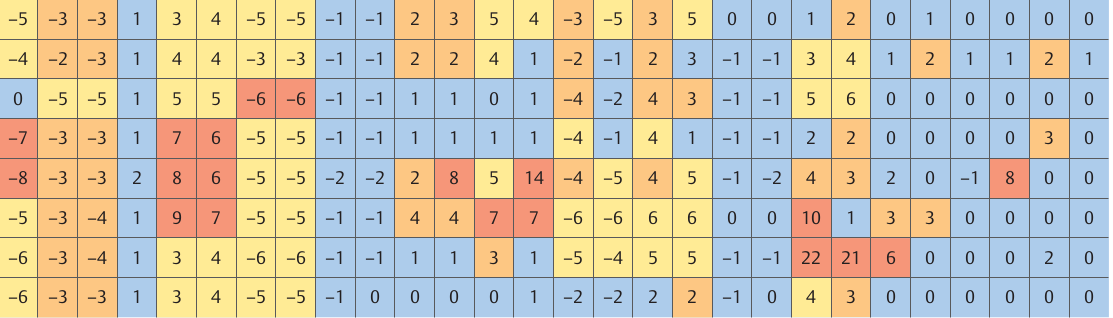
\includegraphics[width=\linewidth]{zmatrix.png}
    \caption{Visualization of common joints between Human3.6M and MPI-INF-3DHP}
    \label{fig:joint-map}
\end{figure}

\subsection{Coordinate frames}

There are two coordinate frames that we consider one is the Camera Coordinate Frame and the other is Hip Coordinate Frame. In the Hip Coordinate Frame the 3D joint positions are placed in a coordinate system where the origin is the Hip joint. The location of all other joints are represented with respect to the hip joint. This representation style encourage the model to learn anthropometric proportions of the human body and estimate more structurally sound estimations. One difficulty with this coordinate frame is that no matter which direction the camera points at the position and orientation of the Hip Coordinate Frame stays constant. This means that the model needs to estimate the orientation of the hip joint very accurately since all other joints depend on the hip joint. Any error made in the estimation of the hip joint orientation would spill into the estimates of all other joints. Please look at \autoref{fig:hip-coordinate} for an example.

\begin{figure}[htpb]
    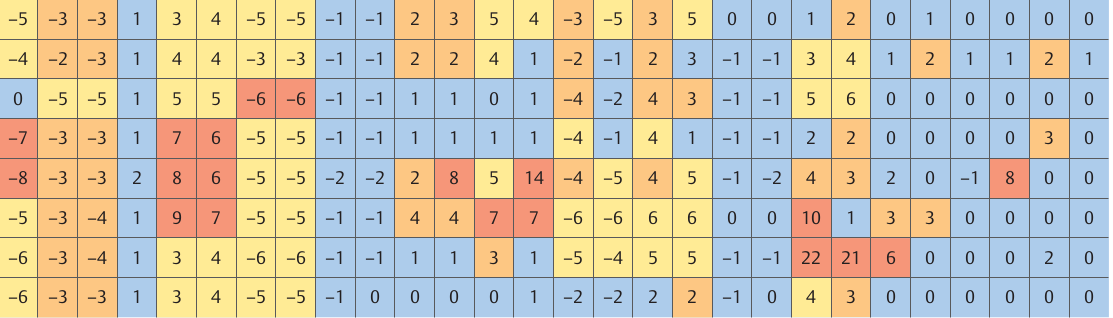
\includegraphics[width=\linewidth]{zmatrix.png}
    \caption{Visualization of the Hip coordinate frame}
    \label{fig:hip-coordinate}
\end{figure}

In the Camera Coordinate Frame the origin is located at the camera position and the z direction points away from the camera. This is a natural coordinate frame to estimate 3D pose since the 2D pose is given from the same coordinate frame. The model needs to accurately estimate the scale that the camera uses which depend on the camera intrinsics and the depth of each joint. Estimating with respect to any other global frame introduces additional problems namely one would need to estimate the position and orientation of both the global coordinate frame and the joints with respect to the camera and apply the necessary transformation to calculate the pose with respect to the global coordinate frame. This complicates the pose estimation procedure unnecessarily.

\subsection{Normalization and the position of the root}

Normalization of the joint positions has tremendous advantages during training. If the data distribution is close to the data distribution during inference this is a clear advantage. However, one needs to be careful when the data distribution during inference is significantly different from the training distribution the accuracy of the estimation will be significantly worsened. We prepared both normalized and raw versions of the dataset to observe the effect of normalization.

One additional normalization strategy is shifting the coordinate frame position to the hip joint which we call rooting. This can be done when estimating the 3D pose in the Camera Coordinate Frame. This has the added benefit that the position of the hip joint doesn't need to be estimated due to the rooting operation and the orientation of the coordinate frame stays the same in contrast to Hip Coordinate Frame where the orientation of the hip joint is a critical estimation step. This step allows the rooted Camera Coordinate Frame to estimate the joint position with respect to an origin which locates in the hip and has the same orientation with the camera. Thus, eliminating the need to estimate two critical parameters.

\section{Feed-Forward Model}

Our aim with this model is to show that viewpoint augmentation can lead the model to increase its prediction accuracy in novel viewpoints. For that we designed a multi-layered Feed-Forward Neural Network with residual connections \parencite{he2016deep} which is inspired by Martinez et. al. \parencite{martinez2017simple}.

\subsection{Network design}

One model is using feed forward network with residual connections in a frame by frame basis. In this model the basic unit is what we call forward unit and it consists of a fully connected layer, followed by a batch norm layer, followed by dropout layers. Another repeating unit is the residual block which consists of 2 forward units and a residual connection from the input of the block to the output of the block. The input frame is passed through a forward unit and then passed through to two residual blocks and a fully connected layer which has 42 units which correspond to 3D position of the 14 joints. For the choice of activation function the effect of using Rectified Linear Units (ReLU) \parencite{nair2010rectified} and Self-normalizing Linear Units (SeLU) \parencite{klambauer2017self} are compared. For the network visualization please see \autoref{fig:feedforward-network}

\begin{figure}[htpb]
    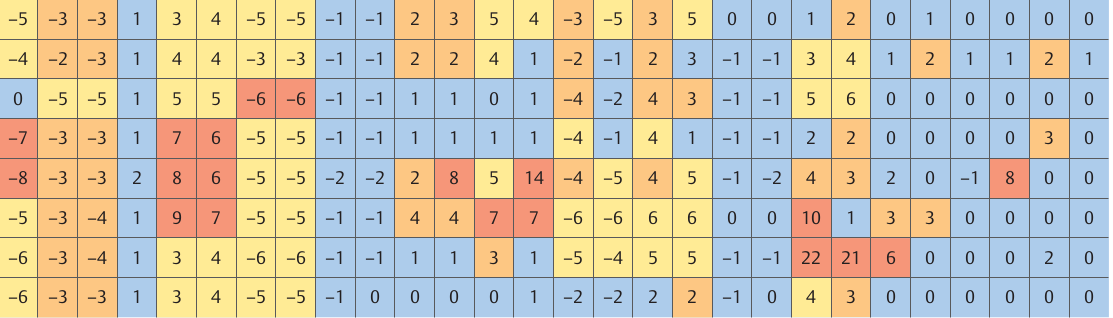
\includegraphics[width=\linewidth]{zmatrix.png}
    \caption{Architecture of the Feed Forward model}
    \label{fig:feedforward-network}
\end{figure}

\subsubsection{Residual connections and Refinement}

Residual connections have the effect of propagating the loss signal without intrusion to earlier layers in the network. This enabled He et. al. \parencite{he2016deep} to train Deep Convolutional Neural Networks which are  152 layers deep giving \%4.49 top-5 error rate. Another way to understand the effect of residual connection is that they smooth out the loss surface and make the optimization much easier as was demonstrated by Li et. al. \parencite{li2017visualizing}.

Newell et. al. \parencite{newell2016stacked} demonstrated that iterative refinement of the 2D joint confidence maps has greatly improved the 2D pose estimation. A similar mechanism is in play in our model with the use of residual connections. All feed forward models share an embedding which the refine over the network. The loss from the final layer propagates to all residual block which can be thought as having many loss functions in between layers. We validate that having residual connections greatly improves prediction accuracy.   

\subsubsection{Batch normalization and dropout}

The effect of Batch normalization \parencite{ioffe2015batch} is not completely understood \parencite{kohler2018towards}. It is widely believed that Batch normalization helps the optimization by reducing internal covariate shift \parencite{ioffe2015batch}. This means that the distribution of the activations in a neural network change during the optimization process due to the change in the wights which is called covariate shift in this scenario. This produces a problem due to the fact that each layer depends on the activations of the previous layer and if the distribution of the activation patterns change than this introduces another signal that the network needs to adapt to. However, evidence that this explanation is incorrect has been recently shown \parencite{santurkar2018does}. Another explanation for the effectiveness of Batch norm is that by decoupling the loss minimization problem into optimizing direction and length of the parameters separately. During training this reduces cross-dependencies between layers and thus simplifies curvature structure and Gradient Descent dynamics \parencite{kohler2018towards}. We observed the effectiveness of using batch-norm in our model.

Dropout \parencite{srivastava2014dropout} has been long known to help to regularize Neural Networks. It works by setting activations in a layer zero with certain probability. This effectively turns the network into an ensemble \parencite{hara2016analysis}. When an input propagates through the network only some neurons and every time the neurons see the input different part of the input and the partial input is seen by different neurons every time due to the random nature of dropout. This introduces an ensemble mechanism which increases the generalization potential by preventing the neurons from memorizing the input output mapping and thus over-fitting. 

\subsubsection{ReLU vs SELU activation}

Rectified Linear Units (ReLU) \parencite{nair2010rectified} have been widely used in Deep Learning due to its effectiveness in preventing the vanishing gradient problem. Earlier activation methods like sigmoids and the hyperbolic tangent function have a small region around zero where the gradient is large. Outside of this active region the gradient of these functions becomes close to zero. This makes training deep networks increasingly difficult since most gradient values cannot propagate to the early layers. However ReLUs don't suffer from this problem and make training very deep networks possible. However they suffer from a different set of problems. ReLUs don't produce an activation for input values which are smaller than zero, this is known as the dead ReLU problem. Moreover, they shift mean of the activations to the positive side which makes the optimization difficult. 

Klambauer et. al. \parencite{klambauer2017self} showed that Scaled Exponential Linear Units (SELU) have a self-normalization characteristic where they preserve the zero mean and unit variance property of the activations. This makes them ideal for training highly robust, deep neural networks. We wanted to test this idea and compare SELU and ReLU activations in our model.

\subsubsection{Viewpoint augmentation}

One of the central points of this model is to test viewpoint invariance. This is achieved through augmentation where the ground truth 3D pose is projected onto multiple virtual cameras placed around the actor in a grid pattern. The pose evaluation is done from a different set of virtual camera positions to validate the viewpoint invariance. % The projection is done using a simple camera model.  Need to add more details

\subsubsection{Loss Function}

Our model estimates the 3D pose $\theta \in R^{3\times N}$ given the 2D pose $X \in R^{2\times N}$. We can represent the neural network as a function $f(x) = y ; x \in R^{2\times N}, y \in R^{3\times N} $. As the loss function we use the L-2 norm between the predicted joint positions and the ground truth joint positions.

\begin{equation}	
    L(f(x),\theta) = \frac{1}{3N} \cdot \sum_{i=1}^{3N} {\Vert f(x_i)-\theta_i \Vert}_2^2
\end{equation}

% Maybe more details

\subsection{Training details}

We trained our model for 100 epochs with batch size is 16384. Large batch training has shown a lot of promise recently \parencite{you2017imagenet}, \parencite{goyal2017accurate}. In our case training with such a high batch size enabled us to train much faster since we could utilize the GPU hardware much more effectively. Adding augmentations meant that we would have much more data to process. For example when using 40 virtual cameras the dataset size for Human3.6M dataset would effectively increase 10 times. This enabled us to train with a faster rate and explore a wider range of architectures and hyper-parameters. We observed that having large batch sizes didn't affect the performance negatively if other hyper-parameters are adjusted as well. For the optimizer we used the ADAM optimizer with learning rate is 0.001. For the wight initialization we used He initialization when training with ReLU activation and SELU activation is initialized with normal distribution with mean zero and variance $\sqrt(2 / n)$ where n denotes number of hidden units in the previous layer. 

\subsection{Evaluation}

We designed an experiment aimed at testing the effectiveness of our augmentation strategy. For the baseline four cameras are used in training and for our model we use 40 views sampled in a grid pattern around the actor. For a visualization please look at \autoref{fig:grid-pattern}. Both models are tested in novel viewpoints and their accuracy is compared. 
Other architectural choices are validated through experiments as well. The activation function is being tested in a second experiment. The effect of normalization, rooting, Camera and Hip centered coordinate frames are also compared. 

\begin{figure}[htpb]
    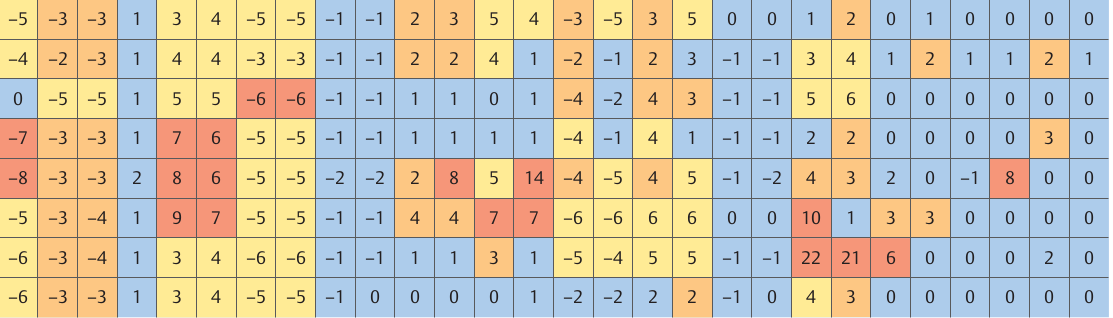
\includegraphics[width=\linewidth]{zmatrix.png}
    \caption{Augmentation through a grid of virtual cameras}
    \label{fig:grid-pattern}
\end{figure}

\subsubsection{Results}

\autoref{tab:feedforward-comp} shows the comparison between a baseline model trained in the original 4 camera views and our model which was trained on 40 virtual camera positions. Evaluation is done in novel camera positions.

\begin{table}[htpb]
    \centering
    \begin{tabular}{l l l l}
        \toprule
            A & B & C & D \\
        \midrule
            1 & 2 & 1 & 2 \\
            2 & 3 & 2 & 3 \\
        \bottomrule
    \end{tabular}
    \caption[Comparison Feed Forward Network]{Compare the viewpoint invariance between standard and augmented Feed Forward Networks}\label{tab:feedforward-comp}
\end{table}



In \autoref{fig:feedforward-compare} the comparative figures can be seen. 

\begin{figure}[htpb]
    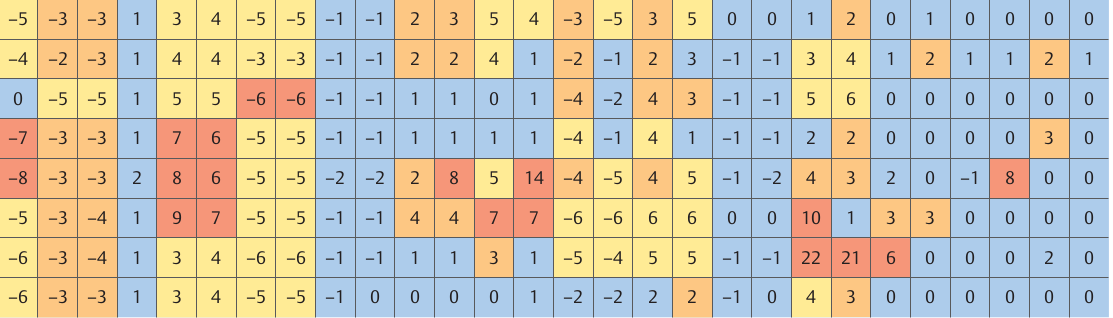
\includegraphics[width=\linewidth]{zmatrix.png}
    \caption{Compariston between of standard and augmented Feed Forward Networks}
    \label{fig:feedforward-compare}
\end{figure}

\subsubsection{Discussion}

It can be seen that training a model with viewpoint augmentation helps become invariant to viewpoint changes.


\section{Temporal Model}

Our aim in this model is to show that a synchronized sequence to sequence model can estimate 3D human pose event when the input 2D pose has missing joints. We architecture that we designed captures the movement pattern of the actor and under circumstances where missing joints are presents interpolates between the previos and future joint positions. This is an important quality of our model in order to give reliable pose estimates in the gait dataset. 

\subsection{Network design}

The second model is exploiting temporal information by using a synchronized sequence to sequence network. Its architectural design is similar to the feed-forward model where instead of the residual block we placed Long-Short-Term-Memory (LSTM) \parencite{hochreiter1997long} cells with recurrent dropout \parencite{semeniuta2016recurrent}. We used Bidirectional Recurrent Neural Network \parencite{schuster1997bidirectional} architecture in order to facilitate not only forward but backward propagation of information as well. This is important since the missing joint can be filled by using 
information from both time directions. They also act as a temporal consistency regularizer combining information from different time steps.

\subsubsection{Synchronized sequence to sequence}

Sequence to sequence models \parencite{sutskever2014sequence} have shown a lot of promising results in Neural Machine Translation \parencite{bahdanau2014neural}, Video Caption Generation \parencite{xu2015show} and Question Answering \parencite{hermann2015teaching}. Their architecture consists of two phases: the encoding phase and the decoding phase. During encoding phase the input sequence is fed to a Recurrent Neural Network and the necessary information is captured inside the hidden state. After a special  symbol is passed which indicates the end of the input sequence the network uses the hidden state to produce and the previous output to produce the current input. Please look at \autoref{fig:sequnce-network} for a visualization. This architecture is very effective especially when used together with an attention mechanism since it can deal with unaligned sequences and sequences of different length.

\begin{figure}[htpb]
    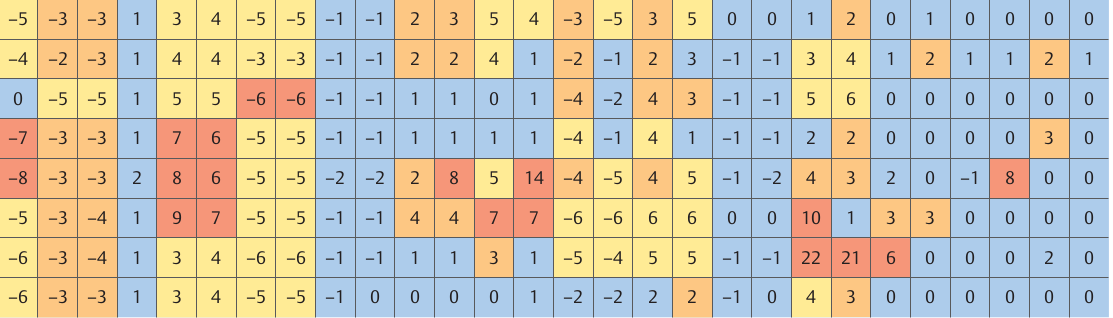
\includegraphics[width=\linewidth]{zmatrix.png}
    \caption{Architecture of the Synchronized Sequence to Sequence Network}
    \label{fig:sequnce-network}
\end{figure}

We use the synchronized sequence to sequence model since we know that the sizes of the two sequences are the same and each 2D pose in the sequence is corresponding to 3D pose element. This makes the connection pattern for the network much simpler. In this architecture the Recurrent Neural Network is fed the input sequence and produces a prediction every time step. The loss is defined for each time step as well.

\subsubsection{Temporal Regularization}

This constraint helps the model enforce temporal regularization. But in order to effectively use this regularization technique we need to divide the joints into three groups as it was suggested by \parencite{hossain2017understanding}. First immobile group which consist of head and hip. Second connection joints which consists of shoulders, knees, and elbows. Lastly, end effectors which include wrists and ankles. This division helps us enforce the movement of the joints in a more fine-grained manner.

\subsubsection{Loss Function}

In this model the both the input and the output are sequences. This leads us to consider the the mean L2 loss across the entire sequence.

\begin{equation}	
    L_2(f(x),\theta) = \frac{1}{3NT} \cdot \sum_{t=1}^{T} \sum_{n=1}^{3N} {\Vert f(x_{n,t})-\theta_{n,t} \Vert}_2^2
\end{equation}

Another loss that we need to account for is the temporal regularization loss which limits the movement of the joints across time.

\begin{equation}	
    L_{temp}(f(x),\theta) = \frac{1}{3NT} \cdot \sum_{t=2}^{T} \sum_{n=1}^{3N} {\Vert f(x_{i,t})-f(x_{i,t-1}) \Vert}_2^2
\end{equation}

so the overall loss becomes 

\begin{equation}	
    L(f(x),\theta) = (1-\alpha) \cdot L_2(f(x),\theta) + \alpha \cdot L_{temp}(f(x),\theta)
\end{equation}

Where $\alpha$ is a hyper-parameter controlling the degree of temporal regularization.

\subsection{Training details}

We train our model for 100 epochs using batch size of 32. We found the sequence length of 128 to be effective. The hyper-parameter for temporal regularization is set to 0.1. We use the ADAM optimizer with learning rate 0.001. 

\subsection{Evaluation}

In order to evaluate the effect our model with respect to missing joint position we artificially remove joints from the input by adding a dropout layer to the beginning of the network. Dropout probability is set to \%10 percent which result in each time step \%10 of the joints being removed from the input. We compare both the feed-forward network and the synchronized sequence to sequence network.

\subsubsection{Results}

For the comparison of the results please look at \autoref{tab:seq-comp}

\begin{table}[htpb]
    \centering
    \begin{tabular}{l l l l}
        \toprule
            A & B & C & D \\
        \midrule
            1 & 2 & 1 & 2 \\
            2 & 3 & 2 & 3 \\
        \bottomrule
    \end{tabular}
    \caption[Comparison Synchronized Sequence to Sequence Network]{Compare the performance in missing joints between Feed Forward Network and Synchronized Sequence to Sequence Network}\label{tab:seq-comp}
\end{table}


Here are examples of pose estimates shown in \autoref{fig:sequence-examples}

\begin{figure}[htpb]
    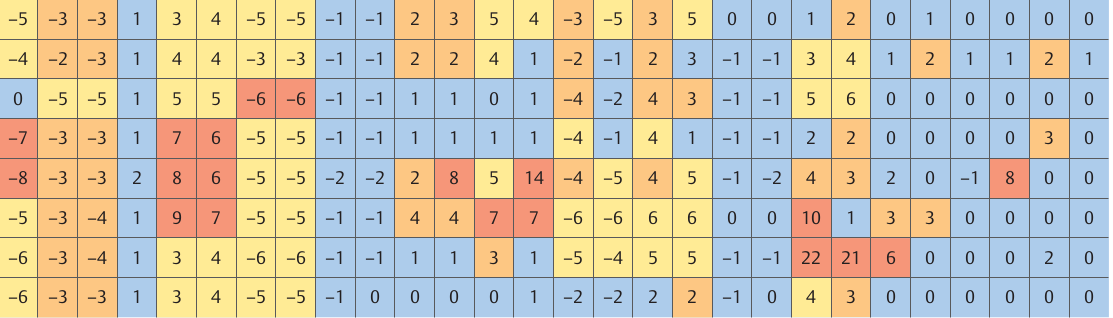
\includegraphics[width=\linewidth]{zmatrix.png}
    \caption{Example 2D inputs 3D ground truth and our model's predictions}
    \label{fig:sequence-examples}
\end{figure}

\subsubsection{Discussion}

Temporal regularization has helped our model to give more stable and noise free 3D pose estimates.


\section{Structural Priors}

Our aim in this model is to constrain the predictions of our model to anthropometrically valid poses and to estimate the skeleton size correctly even when the distance between the subject and the camera changes during the input sequence. This lead us to incorporate additional inputs like the persons height and leg length and additional loss functions.

\subsection{Network design}

The third model is using additional height information together with a loss function which preserves the lengths of the bones. Additional information about the height helps solve the ambiguity relating to distance and size of the body. Additionally it help the network to work for people with different body sizes and body compositions. Bone length loss helps the network estimate the length of bones and makes sure it stays constant during the sequence. 3D pose estimation is an ill-defined problem on its own however these additional priors and data help the network disambiguate challenging poses.

\subsubsection{Bone length loss}

Our main observation in this model is that the length of human bones don't change during a short amount of time. A moving person's apparent size may change when moving towards or away from an observer but this doesn't mean that the size of the person's skeleton is changing. This simple observation lead us to add the notion of bones to our model. We strictly enforce the size of them not to change during the estimation sequence.

\subsubsection{Height and anthropometry}

Another important observation is that just by using the height and leg length of a person bone lengths of a person can be estimated with reasonably high accuracy. This stems from the fact that anthropometric proportions of the human body are relatively stable across people. This assumption is of course not correct but still practical in our case since we require to estimate the 3D pose of a moving person with drastically different visual appearances due to the movement. This forces us to estimate the distance and person size and this assumption helps us achieve this goal.

\subsubsection{Loss Function}

The loss function that we use is similar to the synchronized sequence to sequence model only we add bone length loss and temporal bone length loss to the overall loss

\subsection{Training details}

The training procedure is similar to the procedure of the synchronized sequence to sequence model. Note that here $ x_{i,t} $ denotes the x,y,z position of the joint.

Bone length loss is defined by
\begin{equation}	
    L_{bone}(B,B) = \frac{1}{NT} \cdot \sum_{t=1}^{T} \sum_{n=1}^{N} {\Vert B_{i,t})-B_{i}) \Vert}_2^2
\end{equation}

Temporal bone length loss is defined by

\begin{equation}	
    L_{bone-temp}(B,B) = \frac{1}{NT} \cdot \sum_{t=1}^{T} \sum_{n=1}^{N} {\Vert B_{i,t})-B_{i,t-1}) \Vert}_2^2
\end{equation}

For the overall loss is defined by

\begin{equation}	
    L(f(x),\theta) = (1-\alpha-\beta-\gamma) \cdot L_2(f(x),\theta) + \alpha \cdot L_{temp}(f(x),\theta) + 
    \beta \cdot L_{bone}(f(x),\theta) + \gamma \cdot L_{bone-temp}(f(x),\theta)
\end{equation}

where $\alpha,\beta,\gamma$ are hyper-parameters

\subsection{Evaluation}

In order to evaluate the effect of our structural priors we compared the anthropometric proportions and body size estimates during the evaluation step between the synchronized sequence to sequence model and our model.

We finally test our full model with temporal regularization, structural priors and viewpoint invariance and compare it against our other models.

\subsubsection{Results}

For the comparison of the results please look at \autoref{tab:structural-comp}

\begin{table}[htpb]
    \centering
    \begin{tabular}{l l l l}
        \toprule
            A & B & C & D \\
        \midrule
            1 & 2 & 1 & 2 \\
            2 & 3 & 2 & 3 \\
        \bottomrule
    \end{tabular}
    \caption[Comparison Structural Sequence Network]{Compare the distance and scale invariance between standard and regularized Sequence Networks}\label{tab:structural-comp}
\end{table}


Here are examples of pose estimates shown in \autoref{fig:structural-examples}

\begin{figure}[htpb]
    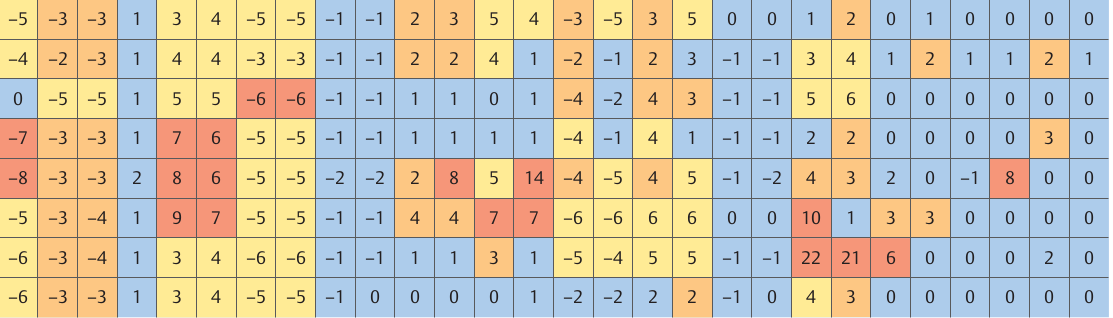
\includegraphics[width=\linewidth]{zmatrix.png}
    \caption{Example 2D inputs 3D ground truth and the Structural Sequence Network's predictions}
    \label{fig:structural-examples}
\end{figure}

Comparison between the final model and previous models are at \autoref{tab:final-comp}

\begin{table}[htpb]
    \centering
    \begin{tabular}{l l l l}
        \toprule
            A & B & C & D \\
        \midrule
            1 & 2 & 1 & 2 \\
            2 & 3 & 2 & 3 \\
        \bottomrule
    \end{tabular}
    \caption[Comparison Final]{Compare the Final Network with augmented Feed Forward Network and augmented Sequence to Sequence Network}\label{tab:final-comp}
\end{table}


Comparative visualizations can be seen in \autoref{fig:final-examples}

\begin{figure}[htpb]
    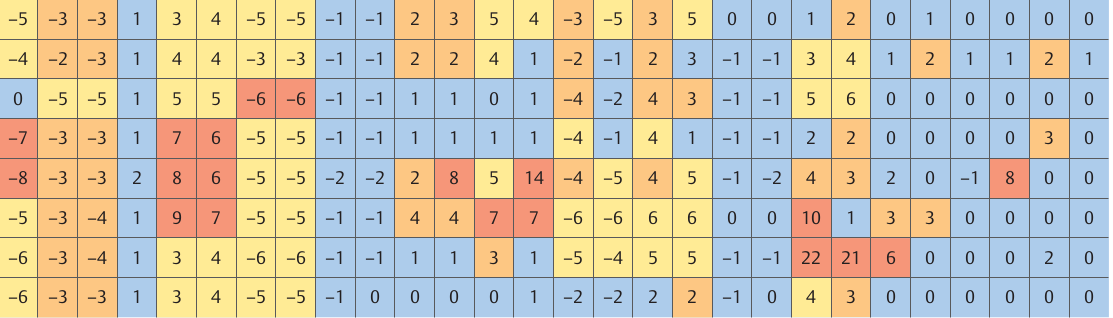
\includegraphics[width=\linewidth]{zmatrix.png}
    \caption{Example 2D inputs 3D ground truth and the Final Network's predictions}
    \label{fig:final-examples}
\end{figure}

\subsubsection{Discussion}

Structural priors gave us better estimation results by incorporating structural elements of the human body and helped in estimating correct scales of skeletons even when the person is moving input sequences.
